\chapter*{Introduction}
\addcontentsline{toc}{chapter}{Introduction}

\hspace{1cm} Réalisé sur un semestre par une équipe de huit à dix étudiants, le projet GE S8 consiste à concevoir une habitation énergétiquement autonome. L'enjeu est de garantir les besoins essentiels de l'utilisateur : éclairage, conservation et cuisson des aliments, la recharge d'appareils électroniques ainsi que le suivi de la production et la consommation d'énergie de l'habitation. Ce premier rapport définit le cadre du projet à travers une analyse fonctionnelle et une étude du cahier des charges. Il détaille également les caractéristiques de la source d'alimentation, qui est une éolienne, et présente l'organisation du travail au sein du groupe.

\section*{Synoptique du Projet}
Pour visualiser l'ensemble du système, voici le synoptique général du projet :
\begin{figure}[H]
    \centering
    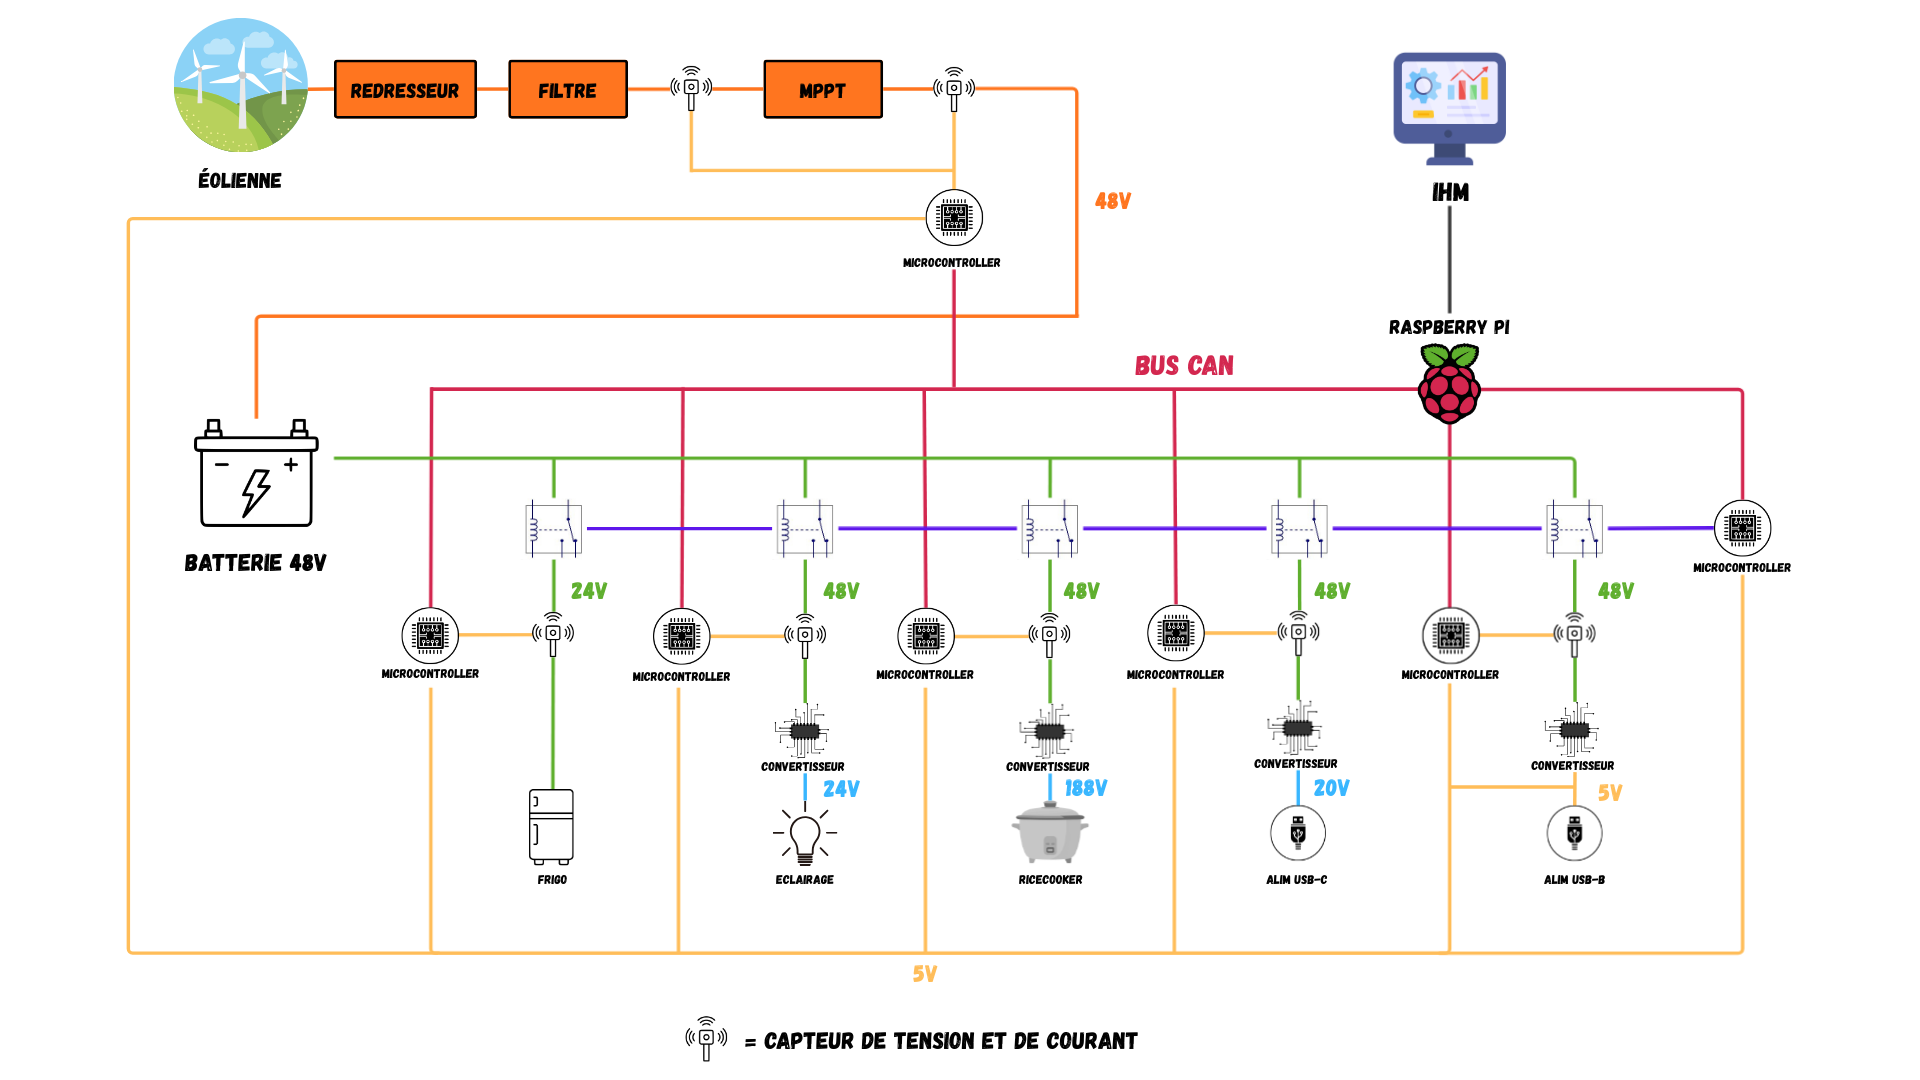
\includegraphics[width=0.9\textwidth]{images/diagrammes/Synoptique projet S8.png}
    \caption{Synoptique du Projet S8}
    \label{fig:synoptique}
\end{figure}

\section*{Organisation de l'équipe}
L'organisation de l'équipe pour ce semestre est présentée ci-dessous :
\begin{figure}[H]
    \centering
    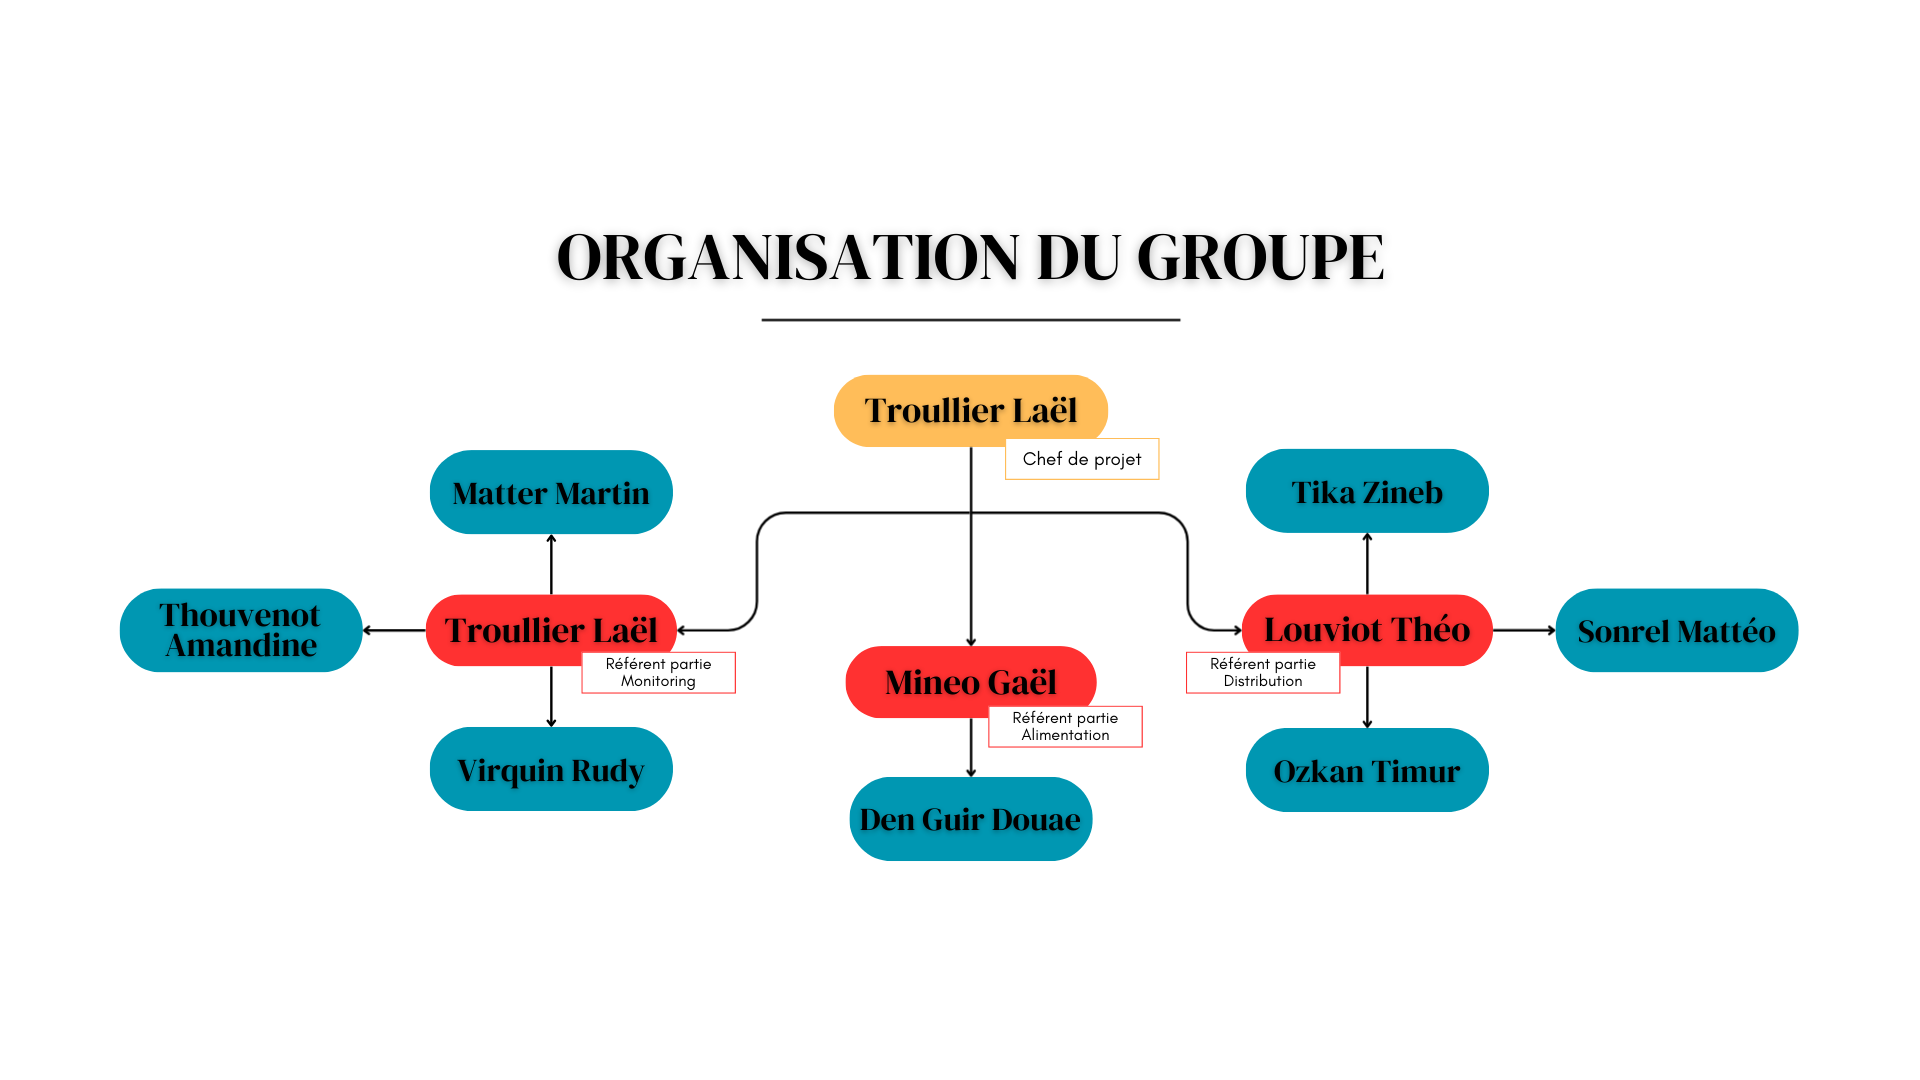
\includegraphics[width=0.9\textwidth]{images/diagrammes/Organigramme Projet S8.png}
    \caption{Organigramme du Projet S8}
    \label{fig:organigramme}
\end{figure}